\chapter{Variables}
\label{s:gui.variables}

\begin{figure}
\centering
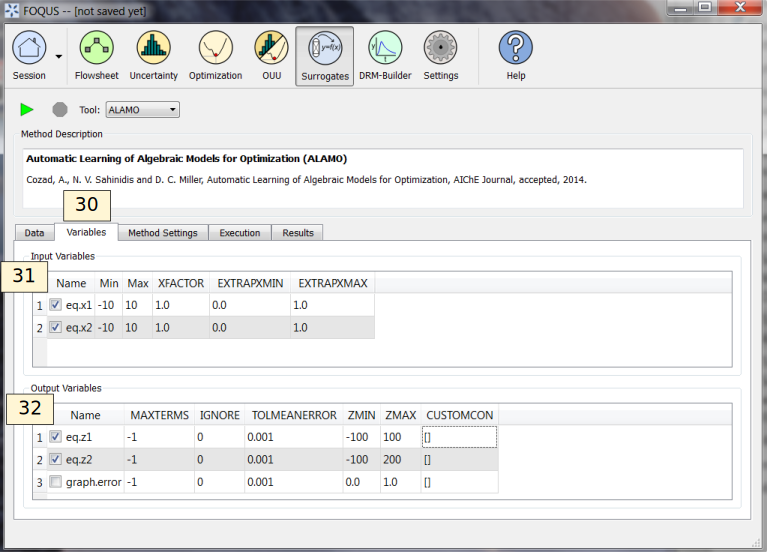
\includegraphics[width=12cm]{figures/variables.pdf}
\caption[The variable viewing and editing windows in the GUI.]{The variable viewing and editing windows in the GUI.
Top middle: accessing the v1 variable window from the root window (console hidden).
Top left: the v1 variable window, showing the currently defined v1 variable arrays.
Bottom left: the variable window for quad_k1, displaying each of its variables and their key attributes.
Middle: the bulk fill window for quad_k1.
Bottom middle: the individual variable window for quad_k1[5], showing all of its settings and allowing the user to edit some of them.
Right: The variable array creation window.}
\label{fig:gui.variables}
\end{figure}

Variables are viewed and edited in the GUI almost exactly the same as data, as shown in Figure \ref{fig:gui.variables}.
An important exception is that, since there are only v1 variables arrays and no v2 arrays of v1 arrays, the variable creation window only has one pane, and separate v1 arrays created in different tabs of the window are completely independent.
Also, the user can clone an existing v1 array with the drop down menu below the "Duplicate" button.

